\documentclass[border=3pt]{standalone}
% Preâmbulo compartilhado pelos diagramas TikZ da aula 7 (Filtros Não Paramétricos)
\usepackage[T1]{fontenc}
\usepackage[utf8]{inputenc}
\usepackage{lmodern}
\usepackage{amsmath}
\usepackage{xcolor}
\usepackage{tikz}
\usetikzlibrary{arrows.meta,angles,quotes,decorations.pathmorphing,calc,
                positioning,shapes.geometric,shapes.misc,backgrounds,fit,
                math}

% Paleta (mesma dos SVGs originais)
\definecolor{dblue}{HTML}{2A5B8C}
\definecolor{dorange}{HTML}{B3541E}
\definecolor{dgreen}{HTML}{4A7C59}
\definecolor{dred}{HTML}{9C4B4B}
\definecolor{dcream}{HTML}{F4F1EA}
\definecolor{dshade}{HTML}{DDD7C9}

% Função gaussiana (não normalizada por padrão de escala visual)
\pgfmathdeclarefunction{gauss}{3}{%
  \pgfmathparse{1/(#3*sqrt(2*pi))*exp(-((#1-#2)^2)/(2*#3^2))}%
}

% Estilos comuns (prefixo d... para não colidir com chaves internas do pgf)
\tikzset{
  >={Stealth[length=2mm]},
  dguide/.style={gray!55, dashed, line width=0.4pt},
  daxis/.style={gray!60, line width=0.7pt, ->},
  dbody/.style={fill=black!3, draw=black!80, line width=1pt},
  dacc/.style={draw=dblue, line width=1pt},
  dlbl/.style={black!55, font=\small},
  dsub/.style={black!45, font=\footnotesize},
  dstate/.style={circle, draw=black!80, fill=dcream, line width=1pt,
                 minimum size=17mm, font=\large, inner sep=1pt},
  dobs/.style={circle, draw=black!80, fill=dshade, line width=1pt,
               minimum size=14mm, font=\large, inner sep=1pt},
  dbox/.style={rounded corners=2pt, draw=black!80, fill=dcream, line width=1pt,
               align=center, inner sep=6pt},
  dop/.style={circle, draw=black!80, fill=white, line width=1pt,
              minimum size=6mm, inner sep=0pt, font=\small},
  dtrans/.style={->, dblue, line width=1pt},
  dmeas/.style={->, dorange, line width=1pt},
  dcurve/.style={line width=1pt, dblue},
  dcurveb/.style={line width=1.4pt, dorange},
}

\begin{document}
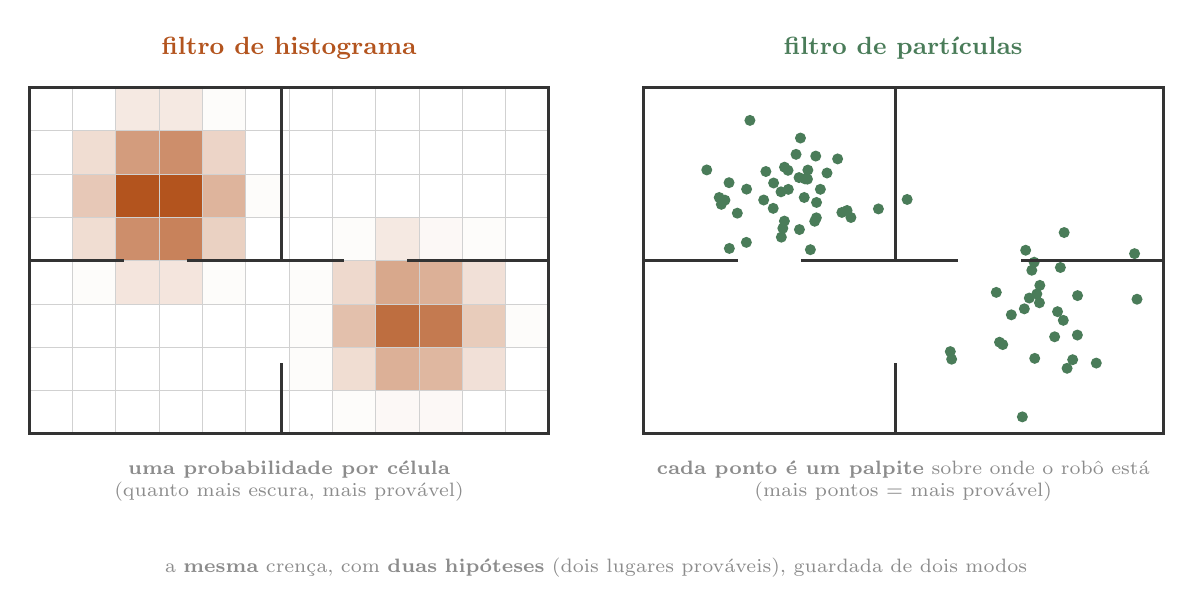
\begin{tikzpicture}[x=1cm,y=1cm]
\node[font=\small\bfseries, dorange] at (3.30,4.90) {filtro de histograma};
\fill[dorange!0, draw=black!18, line width=0.25pt] (0.000,0.000) rectangle ++(0.550,0.550);
\fill[dorange!0, draw=black!18, line width=0.25pt] (0.000,0.550) rectangle ++(0.550,0.550);
\fill[dorange!0, draw=black!18, line width=0.25pt] (0.000,1.100) rectangle ++(0.550,0.550);
\fill[dorange!0, draw=black!18, line width=0.25pt] (0.000,1.650) rectangle ++(0.550,0.550);
\fill[dorange!0, draw=black!18, line width=0.25pt] (0.000,2.200) rectangle ++(0.550,0.550);
\fill[dorange!0, draw=black!18, line width=0.25pt] (0.000,2.750) rectangle ++(0.550,0.550);
\fill[dorange!0, draw=black!18, line width=0.25pt] (0.000,3.300) rectangle ++(0.550,0.550);
\fill[dorange!0, draw=black!18, line width=0.25pt] (0.000,3.850) rectangle ++(0.550,0.550);
\fill[dorange!0, draw=black!18, line width=0.25pt] (0.550,0.000) rectangle ++(0.550,0.550);
\fill[dorange!0, draw=black!18, line width=0.25pt] (0.550,0.550) rectangle ++(0.550,0.550);
\fill[dorange!0, draw=black!18, line width=0.25pt] (0.550,1.100) rectangle ++(0.550,0.550);
\fill[dorange!2, draw=black!18, line width=0.25pt] (0.550,1.650) rectangle ++(0.550,0.550);
\fill[dorange!20, draw=black!18, line width=0.25pt] (0.550,2.200) rectangle ++(0.550,0.550);
\fill[dorange!32, draw=black!18, line width=0.25pt] (0.550,2.750) rectangle ++(0.550,0.550);
\fill[dorange!20, draw=black!18, line width=0.25pt] (0.550,3.300) rectangle ++(0.550,0.550);
\fill[dorange!0, draw=black!18, line width=0.25pt] (0.550,3.850) rectangle ++(0.550,0.550);
\fill[dorange!0, draw=black!18, line width=0.25pt] (1.100,0.000) rectangle ++(0.550,0.550);
\fill[dorange!0, draw=black!18, line width=0.25pt] (1.100,0.550) rectangle ++(0.550,0.550);
\fill[dorange!0, draw=black!18, line width=0.25pt] (1.100,1.100) rectangle ++(0.550,0.550);
\fill[dorange!15, draw=black!18, line width=0.25pt] (1.100,1.650) rectangle ++(0.550,0.550);
\fill[dorange!66, draw=black!18, line width=0.25pt] (1.100,2.200) rectangle ++(0.550,0.550);
\fill[dorange!100, draw=black!18, line width=0.25pt] (1.100,2.750) rectangle ++(0.550,0.550);
\fill[dorange!58, draw=black!18, line width=0.25pt] (1.100,3.300) rectangle ++(0.550,0.550);
\fill[dorange!13, draw=black!18, line width=0.25pt] (1.100,3.850) rectangle ++(0.550,0.550);
\fill[dorange!0, draw=black!18, line width=0.25pt] (1.650,0.000) rectangle ++(0.550,0.550);
\fill[dorange!0, draw=black!18, line width=0.25pt] (1.650,0.550) rectangle ++(0.550,0.550);
\fill[dorange!0, draw=black!18, line width=0.25pt] (1.650,1.100) rectangle ++(0.550,0.550);
\fill[dorange!15, draw=black!18, line width=0.25pt] (1.650,1.650) rectangle ++(0.550,0.550);
\fill[dorange!73, draw=black!18, line width=0.25pt] (1.650,2.200) rectangle ++(0.550,0.550);
\fill[dorange!100, draw=black!18, line width=0.25pt] (1.650,2.750) rectangle ++(0.550,0.550);
\fill[dorange!66, draw=black!18, line width=0.25pt] (1.650,3.300) rectangle ++(0.550,0.550);
\fill[dorange!13, draw=black!18, line width=0.25pt] (1.650,3.850) rectangle ++(0.550,0.550);
\fill[dorange!0, draw=black!18, line width=0.25pt] (2.200,0.000) rectangle ++(0.550,0.550);
\fill[dorange!0, draw=black!18, line width=0.25pt] (2.200,0.550) rectangle ++(0.550,0.550);
\fill[dorange!0, draw=black!18, line width=0.25pt] (2.200,1.100) rectangle ++(0.550,0.550);
\fill[dorange!2, draw=black!18, line width=0.25pt] (2.200,1.650) rectangle ++(0.550,0.550);
\fill[dorange!27, draw=black!18, line width=0.25pt] (2.200,2.200) rectangle ++(0.550,0.550);
\fill[dorange!44, draw=black!18, line width=0.25pt] (2.200,2.750) rectangle ++(0.550,0.550);
\fill[dorange!25, draw=black!18, line width=0.25pt] (2.200,3.300) rectangle ++(0.550,0.550);
\fill[dorange!2, draw=black!18, line width=0.25pt] (2.200,3.850) rectangle ++(0.550,0.550);
\fill[dorange!0, draw=black!18, line width=0.25pt] (2.750,0.000) rectangle ++(0.550,0.550);
\fill[dorange!0, draw=black!18, line width=0.25pt] (2.750,0.550) rectangle ++(0.550,0.550);
\fill[dorange!0, draw=black!18, line width=0.25pt] (2.750,1.100) rectangle ++(0.550,0.550);
\fill[dorange!0, draw=black!18, line width=0.25pt] (2.750,1.650) rectangle ++(0.550,0.550);
\fill[dorange!0, draw=black!18, line width=0.25pt] (2.750,2.200) rectangle ++(0.550,0.550);
\fill[dorange!2, draw=black!18, line width=0.25pt] (2.750,2.750) rectangle ++(0.550,0.550);
\fill[dorange!0, draw=black!18, line width=0.25pt] (2.750,3.300) rectangle ++(0.550,0.550);
\fill[dorange!0, draw=black!18, line width=0.25pt] (2.750,3.850) rectangle ++(0.550,0.550);
\fill[dorange!0, draw=black!18, line width=0.25pt] (3.300,0.000) rectangle ++(0.550,0.550);
\fill[dorange!2, draw=black!18, line width=0.25pt] (3.300,0.550) rectangle ++(0.550,0.550);
\fill[dorange!2, draw=black!18, line width=0.25pt] (3.300,1.100) rectangle ++(0.550,0.550);
\fill[dorange!2, draw=black!18, line width=0.25pt] (3.300,1.650) rectangle ++(0.550,0.550);
\fill[dorange!0, draw=black!18, line width=0.25pt] (3.300,2.200) rectangle ++(0.550,0.550);
\fill[dorange!0, draw=black!18, line width=0.25pt] (3.300,2.750) rectangle ++(0.550,0.550);
\fill[dorange!0, draw=black!18, line width=0.25pt] (3.300,3.300) rectangle ++(0.550,0.550);
\fill[dorange!0, draw=black!18, line width=0.25pt] (3.300,3.850) rectangle ++(0.550,0.550);
\fill[dorange!2, draw=black!18, line width=0.25pt] (3.850,0.000) rectangle ++(0.550,0.550);
\fill[dorange!20, draw=black!18, line width=0.25pt] (3.850,0.550) rectangle ++(0.550,0.550);
\fill[dorange!37, draw=black!18, line width=0.25pt] (3.850,1.100) rectangle ++(0.550,0.550);
\fill[dorange!22, draw=black!18, line width=0.25pt] (3.850,1.650) rectangle ++(0.550,0.550);
\fill[dorange!2, draw=black!18, line width=0.25pt] (3.850,2.200) rectangle ++(0.550,0.550);
\fill[dorange!0, draw=black!18, line width=0.25pt] (3.850,2.750) rectangle ++(0.550,0.550);
\fill[dorange!0, draw=black!18, line width=0.25pt] (3.850,3.300) rectangle ++(0.550,0.550);
\fill[dorange!0, draw=black!18, line width=0.25pt] (3.850,3.850) rectangle ++(0.550,0.550);
\fill[dorange!4, draw=black!18, line width=0.25pt] (4.400,0.000) rectangle ++(0.550,0.550);
\fill[dorange!46, draw=black!18, line width=0.25pt] (4.400,0.550) rectangle ++(0.550,0.550);
\fill[dorange!85, draw=black!18, line width=0.25pt] (4.400,1.100) rectangle ++(0.550,0.550);
\fill[dorange!51, draw=black!18, line width=0.25pt] (4.400,1.650) rectangle ++(0.550,0.550);
\fill[dorange!13, draw=black!18, line width=0.25pt] (4.400,2.200) rectangle ++(0.550,0.550);
\fill[dorange!0, draw=black!18, line width=0.25pt] (4.400,2.750) rectangle ++(0.550,0.550);
\fill[dorange!0, draw=black!18, line width=0.25pt] (4.400,3.300) rectangle ++(0.550,0.550);
\fill[dorange!0, draw=black!18, line width=0.25pt] (4.400,3.850) rectangle ++(0.550,0.550);
\fill[dorange!4, draw=black!18, line width=0.25pt] (4.950,0.000) rectangle ++(0.550,0.550);
\fill[dorange!42, draw=black!18, line width=0.25pt] (4.950,0.550) rectangle ++(0.550,0.550);
\fill[dorange!78, draw=black!18, line width=0.25pt] (4.950,1.100) rectangle ++(0.550,0.550);
\fill[dorange!46, draw=black!18, line width=0.25pt] (4.950,1.650) rectangle ++(0.550,0.550);
\fill[dorange!4, draw=black!18, line width=0.25pt] (4.950,2.200) rectangle ++(0.550,0.550);
\fill[dorange!0, draw=black!18, line width=0.25pt] (4.950,2.750) rectangle ++(0.550,0.550);
\fill[dorange!0, draw=black!18, line width=0.25pt] (4.950,3.300) rectangle ++(0.550,0.550);
\fill[dorange!0, draw=black!18, line width=0.25pt] (4.950,3.850) rectangle ++(0.550,0.550);
\fill[dorange!0, draw=black!18, line width=0.25pt] (5.500,0.000) rectangle ++(0.550,0.550);
\fill[dorange!18, draw=black!18, line width=0.25pt] (5.500,0.550) rectangle ++(0.550,0.550);
\fill[dorange!30, draw=black!18, line width=0.25pt] (5.500,1.100) rectangle ++(0.550,0.550);
\fill[dorange!18, draw=black!18, line width=0.25pt] (5.500,1.650) rectangle ++(0.550,0.550);
\fill[dorange!2, draw=black!18, line width=0.25pt] (5.500,2.200) rectangle ++(0.550,0.550);
\fill[dorange!0, draw=black!18, line width=0.25pt] (5.500,2.750) rectangle ++(0.550,0.550);
\fill[dorange!0, draw=black!18, line width=0.25pt] (5.500,3.300) rectangle ++(0.550,0.550);
\fill[dorange!0, draw=black!18, line width=0.25pt] (5.500,3.850) rectangle ++(0.550,0.550);
\fill[dorange!0, draw=black!18, line width=0.25pt] (6.050,0.000) rectangle ++(0.550,0.550);
\fill[dorange!0, draw=black!18, line width=0.25pt] (6.050,0.550) rectangle ++(0.550,0.550);
\fill[dorange!2, draw=black!18, line width=0.25pt] (6.050,1.100) rectangle ++(0.550,0.550);
\fill[dorange!0, draw=black!18, line width=0.25pt] (6.050,1.650) rectangle ++(0.550,0.550);
\fill[dorange!0, draw=black!18, line width=0.25pt] (6.050,2.200) rectangle ++(0.550,0.550);
\fill[dorange!0, draw=black!18, line width=0.25pt] (6.050,2.750) rectangle ++(0.550,0.550);
\fill[dorange!0, draw=black!18, line width=0.25pt] (6.050,3.300) rectangle ++(0.550,0.550);
\fill[dorange!0, draw=black!18, line width=0.25pt] (6.050,3.850) rectangle ++(0.550,0.550);
\draw[black!80, fill=none, line width=1.1pt] (0,0) rectangle (6.6,4.4);
\draw[dbody, line width=1.1pt] (0,2.2) -- (1.2,2.2) (2.0,2.2) -- (4.0,2.2) (4.8,2.2) -- (6.6,2.2);
\draw[dbody, line width=1.1pt] (3.2,2.2) -- (3.2,4.4) (3.2,0) -- (3.2,0.9);
\node[dsub, font=\scriptsize, align=center] at (3.30,-0.6) {\textbf{uma probabilidade por célula}\\ (quanto mais escura, mais provável)};
\begin{scope}[shift={(7.80,0)}]
\node[font=\small\bfseries, dgreen] at (3.30,4.90) {filtro de partículas};
\draw[dbody, fill=white, line width=1.1pt] (0,0) rectangle (6.6,4.4);
\fill[dgreen] (1.088,3.189) circle (0.07);
\fill[dgreen] (2.197,2.743) circle (0.07);
\fill[dgreen] (1.036,2.967) circle (0.07);
\fill[dgreen] (1.939,3.549) circle (0.07);
\fill[dgreen] (1.092,2.354) circle (0.07);
\fill[dgreen] (2.053,3.237) circle (0.07);
\fill[dgreen] (2.467,3.491) circle (0.07);
\fill[dgreen] (1.649,2.863) circle (0.07);
\fill[dgreen] (2.985,2.856) circle (0.07);
\fill[dgreen] (1.308,2.431) circle (0.07);
\fill[dgreen] (1.748,3.073) circle (0.07);
\fill[dgreen] (1.528,2.969) circle (0.07);
\fill[dgreen] (1.837,3.346) circle (0.07);
\fill[dgreen] (2.248,3.105) circle (0.07);
\fill[dgreen] (0.805,3.351) circle (0.07);
\fill[dgreen] (0.990,2.914) circle (0.07);
\fill[dgreen] (0.963,3.001) circle (0.07);
\fill[dgreen] (1.311,3.107) circle (0.07);
\fill[dgreen] (3.350,2.976) circle (0.07);
\fill[dgreen] (2.121,2.338) circle (0.07);
\fill[dgreen] (1.556,3.331) circle (0.07);
\fill[dgreen] (1.654,3.185) circle (0.07);
\fill[dgreen] (1.752,2.497) circle (0.07);
\fill[dgreen] (1.982,2.594) circle (0.07);
\fill[dgreen] (2.636,2.747) circle (0.07);
\fill[dgreen] (2.043,3.001) circle (0.07);
\fill[dgreen] (2.176,2.699) circle (0.07);
\fill[dgreen] (2.199,2.938) circle (0.07);
\fill[dgreen] (2.332,3.312) circle (0.07);
\fill[dgreen] (1.771,2.610) circle (0.07);
\fill[dgreen] (2.084,3.234) circle (0.07);
\fill[dgreen] (2.521,2.811) circle (0.07);
\fill[dgreen] (1.977,3.254) circle (0.07);
\fill[dgreen] (1.841,3.104) circle (0.07);
\fill[dgreen] (1.791,2.701) circle (0.07);
\fill[dgreen] (1.193,2.802) circle (0.07);
\fill[dgreen] (1.995,3.756) circle (0.07);
\fill[dgreen] (2.189,3.527) circle (0.07);
\fill[dgreen] (2.089,3.349) circle (0.07);
\fill[dgreen] (1.792,3.386) circle (0.07);
\fill[dgreen] (2.587,2.836) circle (0.07);
\fill[dgreen] (1.353,3.980) circle (0.07);
\fill[dgreen] (5.035,1.885) circle (0.07);
\fill[dgreen] (5.381,0.832) circle (0.07);
\fill[dgreen] (6.238,2.288) circle (0.07);
\fill[dgreen] (4.997,1.776) circle (0.07);
\fill[dgreen] (4.970,0.958) circle (0.07);
\fill[dgreen] (4.838,1.587) circle (0.07);
\fill[dgreen] (5.514,1.755) circle (0.07);
\fill[dgreen] (4.933,2.077) circle (0.07);
\fill[dgreen] (4.482,1.796) circle (0.07);
\fill[dgreen] (5.512,1.254) circle (0.07);
\fill[dgreen] (3.915,0.947) circle (0.07);
\fill[dgreen] (5.030,1.664) circle (0.07);
\fill[dgreen] (5.752,0.898) circle (0.07);
\fill[dgreen] (4.901,1.724) circle (0.07);
\fill[dgreen] (4.813,0.215) circle (0.07);
\fill[dgreen] (5.344,2.556) circle (0.07);
\fill[dgreen] (5.452,0.941) circle (0.07);
\fill[dgreen] (4.673,1.511) circle (0.07);
\fill[dgreen] (6.269,1.709) circle (0.07);
\fill[dgreen] (4.963,2.179) circle (0.07);
\fill[dgreen] (4.855,2.331) circle (0.07);
\fill[dgreen] (4.523,1.163) circle (0.07);
\fill[dgreen] (5.296,2.112) circle (0.07);
\fill[dgreen] (5.260,1.551) circle (0.07);
\fill[dgreen] (3.898,1.044) circle (0.07);
\fill[dgreen] (4.564,1.133) circle (0.07);
\fill[dgreen] (5.223,1.232) circle (0.07);
\fill[dgreen] (5.333,1.441) circle (0.07);

\draw[dbody, line width=1.1pt] (0,2.2) -- (1.2,2.2) (2.0,2.2) -- (4.0,2.2) (4.8,2.2) -- (6.6,2.2);
\draw[dbody, line width=1.1pt] (3.2,2.2) -- (3.2,4.4) (3.2,0) -- (3.2,0.9);
\node[dsub, font=\scriptsize, align=center] at (3.30,-0.6) {\textbf{cada ponto é um palpite} sobre onde o robô está\\ (mais pontos = mais provável)};
\end{scope}
\node[dsub, font=\scriptsize, align=center, text width=14cm] at (7.20,-1.7) {a \textbf{mesma} crença, com \textbf{duas hipóteses} (dois lugares prováveis), guardada de dois modos};
\end{tikzpicture}
\end{document}
